\documentclass[aspectratio=169,11pt]{beamer}
\usepackage[T1]{fontenc}
\usepackage[utf8]{inputenc}
\usepackage[provide=*,french]{babel}
\usepackage{lmodern}
\usepackage{tikz}
\usetikzlibrary{arrows.meta,positioning,calc,shapes.geometric}
\usepackage{hyperref}
\definecolor{vert}{HTML}{1C322D}
\definecolor{creme}{HTML}{F8F3EE}
\definecolor{or}{HTML}{EBB552}
\definecolor{rose}{HTML}{F1CDBE}
\setbeamercolor{normal text}{fg=creme,bg=vert}
\setbeamercolor{frametitle}{fg=creme,bg=vert}
\setbeamercolor{title}{fg=creme}
\setbeamercolor{structure}{fg=or}
\setbeamercolor{block title}{fg=vert,bg=or}
\setbeamercolor{block body}{fg=vert,bg=creme}
\setbeamertemplate{navigation symbols}{}
\setbeamertemplate{footline}{\hfill\color{creme!65}\scriptsize SNT · Le Web · Séance 4\quad\insertframenumber\,/\,\inserttotalframenumber\hspace{5mm}\vspace{3mm}}
\setbeamertemplate{frametitle}{\vspace{3mm}\insertframetitle\par\vspace{2mm}\color{or}\rule{\linewidth}{.6pt}}
\setbeamersize{text margin left=9mm,text margin right=9mm}
\newcommand{\question}[1]{{\Large\color{or}\bfseries #1}}
\newcommand{\reperes}[1]{\vfill{\color{rose}\footnotesize À faire formuler : }{\footnotesize #1}}
\tikzset{boite/.style={draw=or,thick,rounded corners=2mm,fill=creme,text=vert,align=center,minimum width=2.4cm,minimum height=1.3cm},fleche/.style={-{Latex[length=3mm]},thick,draw=or}}
\title{Chercher, publier, se protéger}
\subtitle{Le Web · Livret 4 · Approche First Principles}
\author{Sciences numériques et technologie · Seconde}
\date{}
\begin{document}

\begin{frame}[plain]
\vspace{1.1cm}
{\color{or}\large SNT · LE WEB · SÉANCE 4}\par\vspace{7mm}
{\Huge\bfseries Chercher, publier, se protéger}\par\vspace{7mm}
{\color{rose}\Large Trois problèmes du quotidien, des règles à construire}\par
\vfill \small Recherche · droit d'auteur · hameçonnage · navigateur
\end{frame}

\begin{frame}{Problème n° 5 : une page sans adresse}
\question{Comment trouver une page dont on ignore l'URL ?}
\vspace{6mm}
\begin{center}
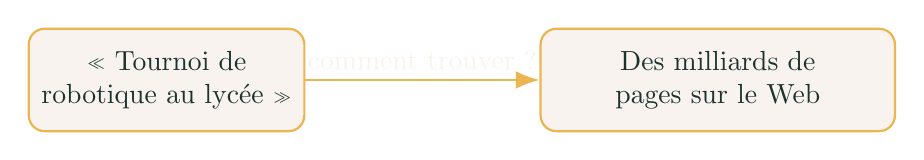
\begin{tikzpicture}
\node[boite,minimum width=3.5cm] (q) at (0,0) {« Tournoi de\\ robotique au lycée »};
\node[boite,minimum width=4.5cm] (w) at (7,0) {Des milliards de\\ pages sur le Web};
\draw[fleche] (q)--node[above,text=creme]{comment trouver ?}(w);
\end{tikzpicture}
\end{center}
\vspace{6mm}
\pause
\begin{block}{L'obstacle}
Il serait beaucoup trop long de parcourir tout le Web au moment où l'on tape chaque recherche.
\end{block}
\reperes{Comment se préparer à répondre très vite ?}
\note{Repartir du problème 5 du livret 1. Laisser les élèves proposer une recherche à l'avance avant d'introduire les mots robot et index.}
\end{frame}

\begin{frame}{Avant la recherche : explorer}
\question{Qui découvre les pages ?}
\vspace{5mm}
\begin{center}
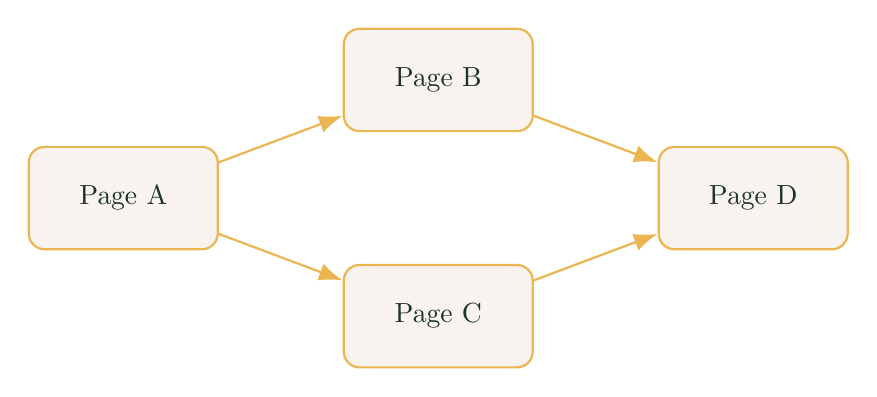
\begin{tikzpicture}
\node[boite] (a) at (0,0) {Page A};
\node[boite] (b) at (4,1.5) {Page B};
\node[boite] (c) at (4,-1.5) {Page C};
\node[boite] (d) at (8,0) {Page D};
\draw[fleche] (a)--(b);\draw[fleche] (a)--(c);
\draw[fleche] (b)--(d);\draw[fleche] (c)--(d);
\end{tikzpicture}
\end{center}
\pause
\begin{block}{Exploration}
Un \textbf{robot} suit les liens et visite des pages pour recueillir leur contenu. Ce travail se poursuit en arrière-plan, indépendamment de ta recherche.
\end{block}
\end{frame}

\begin{frame}{Retrouver rapidement les pages}
\question{Comment retrouver un mot sans relire tous les documents ?}
\vspace{2mm}
\begin{center}
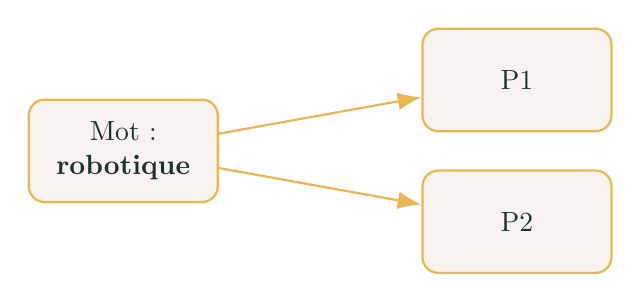
\begin{tikzpicture}
\node[boite] (m) at (0,0) {Mot :\\ \textbf{robotique}};
\node[boite] (p1) at (5,.9) {P1};
\node[boite] (p2) at (5,-.9) {P2};
\draw[fleche] (m)--(p1);\draw[fleche] (m)--(p2);
\end{tikzpicture}
\end{center}
\pause
\begin{block}{Index}
Comme à la fin d'un livre, un \textbf{index} associe les mots aux pages qui les contiennent.
\end{block}
\reperes{Dans quelles pages du livret apparaît le mot « tournoi » ?}
\end{frame}

\begin{frame}{Activité 4.1 : indexer à la main}
\question{Et si nous étions un moteur de recherche ?}
\vspace{6mm}
\begin{enumerate}\setlength{\itemsep}{5mm}
\item Lire trois mini-pages.
\item Construire la liste des pages contenant chaque mot.
\item Chercher « tournoi robotique ».
\item Comparer avec « inscriptions mars ».
\end{enumerate}
\vfill
\begin{center}{\Large\color{or}\bfseries Livret 4 · Activité 4.1}\end{center}
\note{Après l'activité, demander pourquoi P1 et P3 ne sont pas nécessairement ex aequo en qualité pour « inscriptions mars ». Faire émerger le classement.}
\end{frame}

\begin{frame}{L'index ne suffit pas}
\question{Deux pages correspondent : laquelle afficher en premier ?}
\vspace{5mm}
\begin{center}
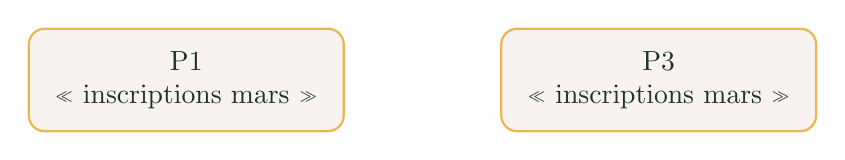
\begin{tikzpicture}
\node[boite,minimum width=4cm] (a) at (0,0) {P1\\ « inscriptions mars »};
\node[boite,minimum width=4cm] (b) at (6,0) {P3\\ « inscriptions mars »};
\end{tikzpicture}
\end{center}
\vspace{5mm}
\pause
\begin{block}{Le nouveau problème}
Plusieurs pages peuvent contenir les mêmes mots. Il faut les \textbf{classer} en tenant compte de critères supplémentaires.
\end{block}
\reperes{Une page citée par beaucoup d'autres serait-elle plus utile ?}
\end{frame}

\begin{frame}{Les liens comme votes}
\question{Une page reçoit trois liens. Une autre n'en reçoit qu'un.}
\vspace{5mm}
\begin{center}
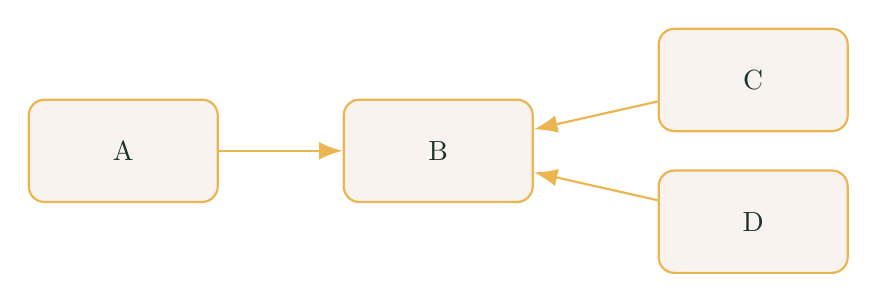
\begin{tikzpicture}
\node[boite] (a) at (0,0) {A}; \node[boite] (b) at (4,0) {B};
\node[boite] (c) at (8,.9) {C}; \node[boite] (d) at (8,-.9) {D};
\draw[fleche] (a)--(b);\draw[fleche] (c)--(b);\draw[fleche] (d)--(b);
\end{tikzpicture}
\end{center}
\pause
\begin{block}{Première intuition}
Les \textbf{liens entrants} peuvent indiquer qu'une page est citée par d'autres. Mais tous les liens n'ont pas la même valeur.
\end{block}
\end{frame}

\begin{frame}{Pourquoi compter les liens ne suffit pas}
\question{Et si je créais 1 000 fausses pages ?}
\vspace{5mm}
\begin{itemize}\setlength{\itemsep}{5mm}
\item Le simple nombre de liens peut être manipulé.
\pause
\item Un lien venant d'une page reconnue peut avoir davantage de poids.
\pause
\item Une page qui crée de nombreux liens partage son poids entre eux.
\end{itemize}
\vspace{6mm}
\begin{block}{Modèle simplifié de PageRank}
Chaque page commence avec un score de 1, puis le partage entre ses liens sortants. Nous allons effectuer \textbf{un seul tour} de calcul.
\end{block}
\end{frame}

\begin{frame}{Activité 4.2 : calcul guidé}
\question{Qui donne du score à qui ?}
\vspace{5mm}
\begin{center}
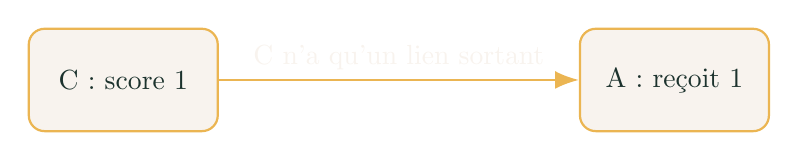
\begin{tikzpicture}
\node[boite] (c) at (0,0) {C : score 1};
\node[boite] (a) at (7,0) {A : reçoit 1};
\draw[fleche] (c)--node[above,text=creme]{C n'a qu'un lien sortant}(a);
\end{tikzpicture}
\end{center}
\vspace{7mm}
\pause
\begin{block}{Méthode}
\textbf{Contribution d'un lien} = score de départ de la page / nombre de ses liens sortants.
\end{block}
\vspace{3mm}
\centering{\color{or}\Large Calculons A ensemble, puis B, C, D et E.}
\note{L'activité se limite volontairement à un tour de partage. Le PageRank réel est itératif et inclut notamment un amortissement.}
\end{frame}

\begin{frame}{Un résultat en premier est-il vrai ?}
\question{Le classement mesure-t-il la fiabilité ?}
\vspace{6mm}
\begin{itemize}\setlength{\itemsep}{6mm}
\item Un lien très consulté peut contenir une erreur.
\pause
\item Un premier résultat peut être une annonce.
\pause
\item Pour un exposé, il faut regarder \textbf{qui parle}, \textbf{quand}, et \textbf{sur quelles preuves}.
\end{itemize}
\vfill
\begin{center}{\Large\color{or}\bfseries Livret 4 · Activité 4.3}\end{center}
\end{frame}

\begin{frame}{Une image trouvée en ligne}
\question{Puis-je la publier sur le site du lycée ?}
\vspace{6mm}
\begin{center}
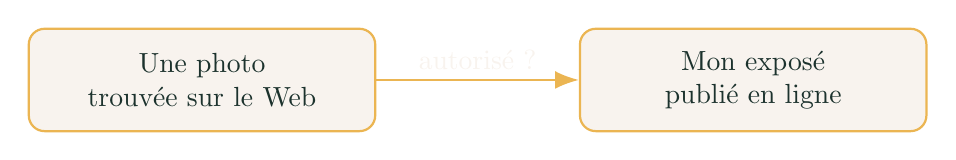
\begin{tikzpicture}
\node[boite,minimum width=4.4cm] (a) at (0,0) {Une photo\\ trouvée sur le Web};
\node[boite,minimum width=4.4cm] (b) at (7,0) {Mon exposé\\ publié en ligne};
\draw[fleche] (a)--node[above,text=creme]{autorisé ?}(b);
\end{tikzpicture}
\end{center}
\pause
\begin{block}{Principe}
Une œuvre originale bénéficie du \textbf{droit d'auteur} dès sa création. Être visible en ligne ne signifie pas « libre à réutiliser ».
\end{block}
\end{frame}

\begin{frame}{Comment partager avec des règles claires ?}
\question{L'auteur peut-il autoriser certaines réutilisations ?}
\vspace{5mm}
\pause
\begin{block}{La licence}
Une \textbf{licence} précise les usages autorisés et les conditions à respecter.
\end{block}
\vspace{6mm}
\begin{description}\setlength{\itemsep}{3mm}
\item[BY] Citer l'auteur et fournir les informations de licence.
\item[NC] Pas d'utilisation commerciale.
\item[ND] Pas de diffusion d'adaptation.
\item[SA] Diffuser une adaptation sous une licence compatible.
\end{description}
\note{Exemple : CC BY-SA. Si la photo est seulement incorporée sans modification, la clause SA ne transforme pas tout l'exposé en CC BY-SA. Voir les textes Creative Commons.}
\end{frame}

\begin{frame}{Acheter un fichier, quels droits ?}
\question{Un e-book acheté se revend-il comme un livre papier ?}
\vspace{6mm}
\begin{itemize}\setlength{\itemsep}{5mm}
\item Pour un livre papier, je possède l'exemplaire matériel.
\pause
\item Pour un téléchargement, la copie reste soumise aux droits et conditions d'utilisation applicables.
\pause
\item Posséder une copie numérique ne signifie pas pouvoir la redistribuer librement.
\end{itemize}
\vfill
\begin{center}{\Large\color{or}\bfseries Livret 4 · Activité 4.4}\end{center}
\note{Nuancer : les règles varient selon le type de fichier, la licence et le contrat. En droit français, les droits patrimoniaux durent en général 70 ans après la mort ; le droit moral demeure.}
\end{frame}

\begin{frame}{Le piège du faux site}
\question{Deux adresses se ressemblent. À laquelle faire confiance ?}
\vspace{5mm}
\begin{block}{Adresse A}
\ttfamily https://www.mabanque.example/compte
\end{block}
\vspace{3mm}
\begin{block}{Adresse B}
\ttfamily https://www.mabanque.example.connexion-securisee.example/compte
\end{block}
\pause
\vspace{5mm}
\centering{\color{or}\Large Le nom de la banque apparaît dans les deux !}
\reperes{Quelle partie indique réellement le site contacté ?}
\end{frame}

\begin{frame}{Lire correctement une URL}
\question{Où se trouve le nom d'hôte ?}
\vspace{5mm}
\begin{center}
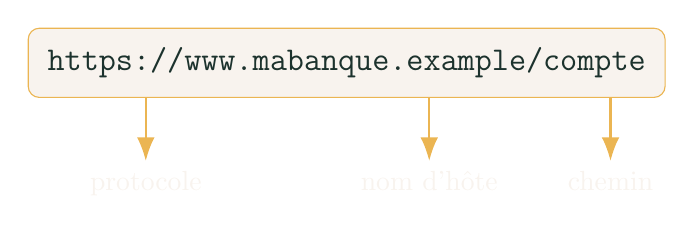
\begin{tikzpicture}
\node[draw=or,fill=creme,text=vert,rounded corners,inner sep=7pt,font=\ttfamily\large] (u) at (0,0) {https://www.mabanque.example/compte};
\draw[fleche] ($(u.south west)+(1.5,0)$)--++(0,-.8) node[below,text=creme,font=\normalsize]{protocole};
\draw[fleche] ($(u.south west)+(5.1,0)$)--++(0,-.8) node[below,text=creme,font=\normalsize]{nom d'hôte};
\draw[fleche] ($(u.south east)+(-.7,0)$)--++(0,-.8) node[below,text=creme,font=\normalsize]{chemin};
\end{tikzpicture}
\end{center}
\vspace{10mm}
\pause
\begin{block}{Méthode}
Après \texttt{https://}, lis jusqu'au prochain \texttt{/}. Identifie ensuite le \textbf{domaine principal} en partant de la droite.
\end{block}
\note{Les étiquettes du diagramme sont approximativement placées sous les trois parties. Insister sur le fait que « www » est un sous-domaine ; le domaine principal attendu est mabanque.example.}
\end{frame}

\begin{frame}{HTTPS garantit-il l'honnêteté ?}
\question{Un faux site peut-il afficher le cadenas ?}
\vspace{6mm}
\begin{center}
{\Huge\color{or}\textbf{HTTPS}}\par\vspace{4mm}
\Large protège la \textbf{communication} avec le site
\end{center}
\pause
\vspace{7mm}
\begin{block}{Mais attention}
Un fraudeur peut lui aussi utiliser HTTPS. Il faut contrôler l'adresse et le contexte de la demande avant de saisir des informations sensibles.
\end{block}
\vfill
\begin{center}{\Large\color{or}\bfseries Livret 4 · Activité 4.5}\end{center}
\end{frame}

\begin{frame}{Pourquoi un site me reconnaît-il ?}
\question{Comment rester connecté en changeant de page ?}
\vspace{6mm}
\begin{center}
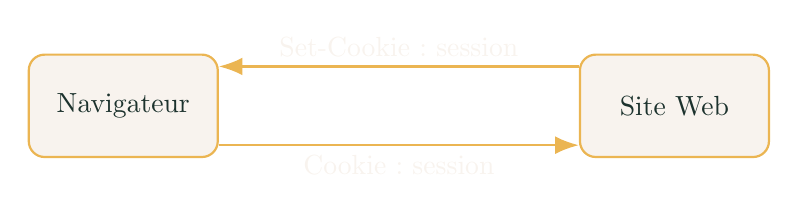
\begin{tikzpicture}
\node[boite] (n) at (0,0) {Navigateur};
\node[boite] (s) at (7,0) {Site Web};
\draw[fleche] ([yshift=5mm]s.west)--node[above,text=creme]{Set-Cookie : session}( [yshift=5mm]n.east);
\pause
\draw[fleche] ([yshift=-5mm]n.east)--node[below,text=creme]{Cookie : session}([yshift=-5mm]s.west);
\end{tikzpicture}
\end{center}
\vspace{7mm}
\begin{block}{Cookie}
Une petite donnée conservée par le navigateur peut aider le site à retrouver la session de l'utilisateur.
\end{block}
\end{frame}

\begin{frame}{Quand le suivi dépasse un seul site}
\question{Pourquoi un même service apparaît-il sur plusieurs sites ?}
\vspace{4mm}
\begin{center}
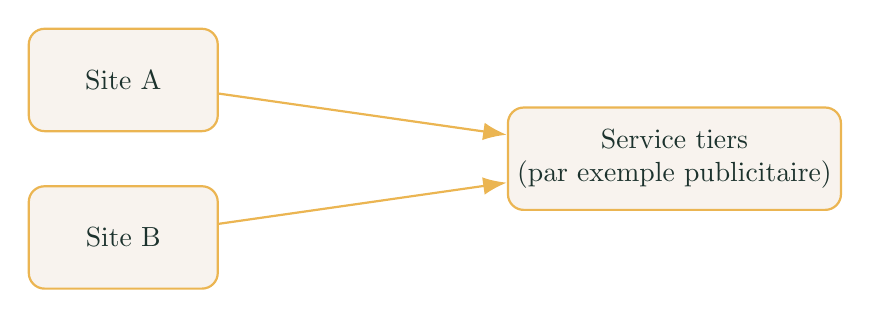
\begin{tikzpicture}
\node[boite] (a) at (0,1) {Site A};
\node[boite] (b) at (0,-1) {Site B};
\node[boite,minimum width=4cm] (t) at (7,0) {Service tiers\\ (par exemple publicitaire)};
\draw[fleche] (a)--(t);\draw[fleche] (b)--(t);
\end{tikzpicture}
\end{center}
\pause
\begin{block}{Pistage}
Certains services tiers peuvent reconnaître un navigateur d'un site à l'autre à l'aide de traceurs. Les protections du navigateur cherchent à limiter ce suivi.
\end{block}
\end{frame}

\begin{frame}{La navigation privée et ses limites}
\question{Qui ne voit plus mes visites ?}
\vspace{6mm}
\begin{itemize}\setlength{\itemsep}{6mm}
\item La navigation privée limite les traces conservées \textbf{sur l'appareil après la session}.
\pause
\item Le site consulté reçoit toujours les requêtes.
\pause
\item Le réseau utilisé peut encore observer des informations sur les connexions.
\end{itemize}
\vspace{4mm}
\begin{block}{En classe}
Dans Firefox : \textbf{Paramètres} puis \textbf{Vie privée et sécurité}. Observer sans modifier irréversiblement les réglages du poste.
\end{block}
\end{frame}

\begin{frame}{Activité 4.6 : observer Firefox}
\question{Que nous montre réellement le navigateur ?}
\vspace{6mm}
\begin{enumerate}\setlength{\itemsep}{6mm}
\item Trouver les options de protection et les autorisations.
\item Ouvrir \textbf{F12} puis \textbf{Stockage} pour observer les cookies visibles.
\item Cliquer sur le \textbf{bouclier} pour lire les protections signalées.
\end{enumerate}
\vspace{4mm}
\pause
\begin{block}{Important}
Cookies stockés, domaines contactés et traqueurs bloqués sont \textbf{trois observations différentes}.
\end{block}
\end{frame}

\begin{frame}{Vérification finale}
\question{Une adresse commence par HTTPS. Est-elle forcément sûre ?}
\vspace{5mm}
\begin{enumerate}[A.]\setlength{\itemsep}{6mm}
\item Oui, le site est nécessairement honnête.
\item Non, HTTPS chiffre la communication mais ne prouve pas l'honnêteté.
\item Oui, si le nom de la banque apparaît quelque part.
\end{enumerate}
\pause
\vspace{5mm}
\begin{block}{Réponse B}
Vérifier le véritable domaine principal et le contexte avant de saisir ses identifiants.
\end{block}
\note{Faire voter sans montrer la dernière apparition.}
\end{frame}

\begin{frame}{Bilan du Web}
\begin{center}
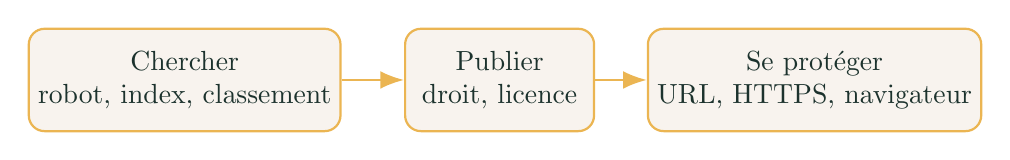
\begin{tikzpicture}
\node[boite] (a) at (0,0) {Chercher\\ robot, index, classement};
\node[boite] (b) at (4,0) {Publier\\ droit, licence};
\node[boite] (c) at (8,0) {Se protéger\\ URL, HTTPS, navigateur};
\draw[fleche] (a)--(b);\draw[fleche] (b)--(c);
\end{tikzpicture}
\end{center}
\vspace{8mm}
\begin{center}
{\color{or}\Large\bfseries Trois questions à retenir}\\par\vspace{3mm}
Comment trouve-t-on une information ?\\[2mm]
Quels droits a-t-on sur une œuvre ?\\[2mm]
Comment vérifier une adresse et limiter ses traces ?
\end{center}
\note{Faire ensuite la frise et les trois tâches d'auto-évaluation du paragraphe 15.}
\end{frame}
\end{document}
